% Marius-Juston 2026
\documentclass[tikz, border=10pt]{standalone}
\usepackage{tikz}
\usepackage{amsmath}
\usetikzlibrary{automata, positioning, arrows.meta, calc, shapes.geometric}

\begin{document}
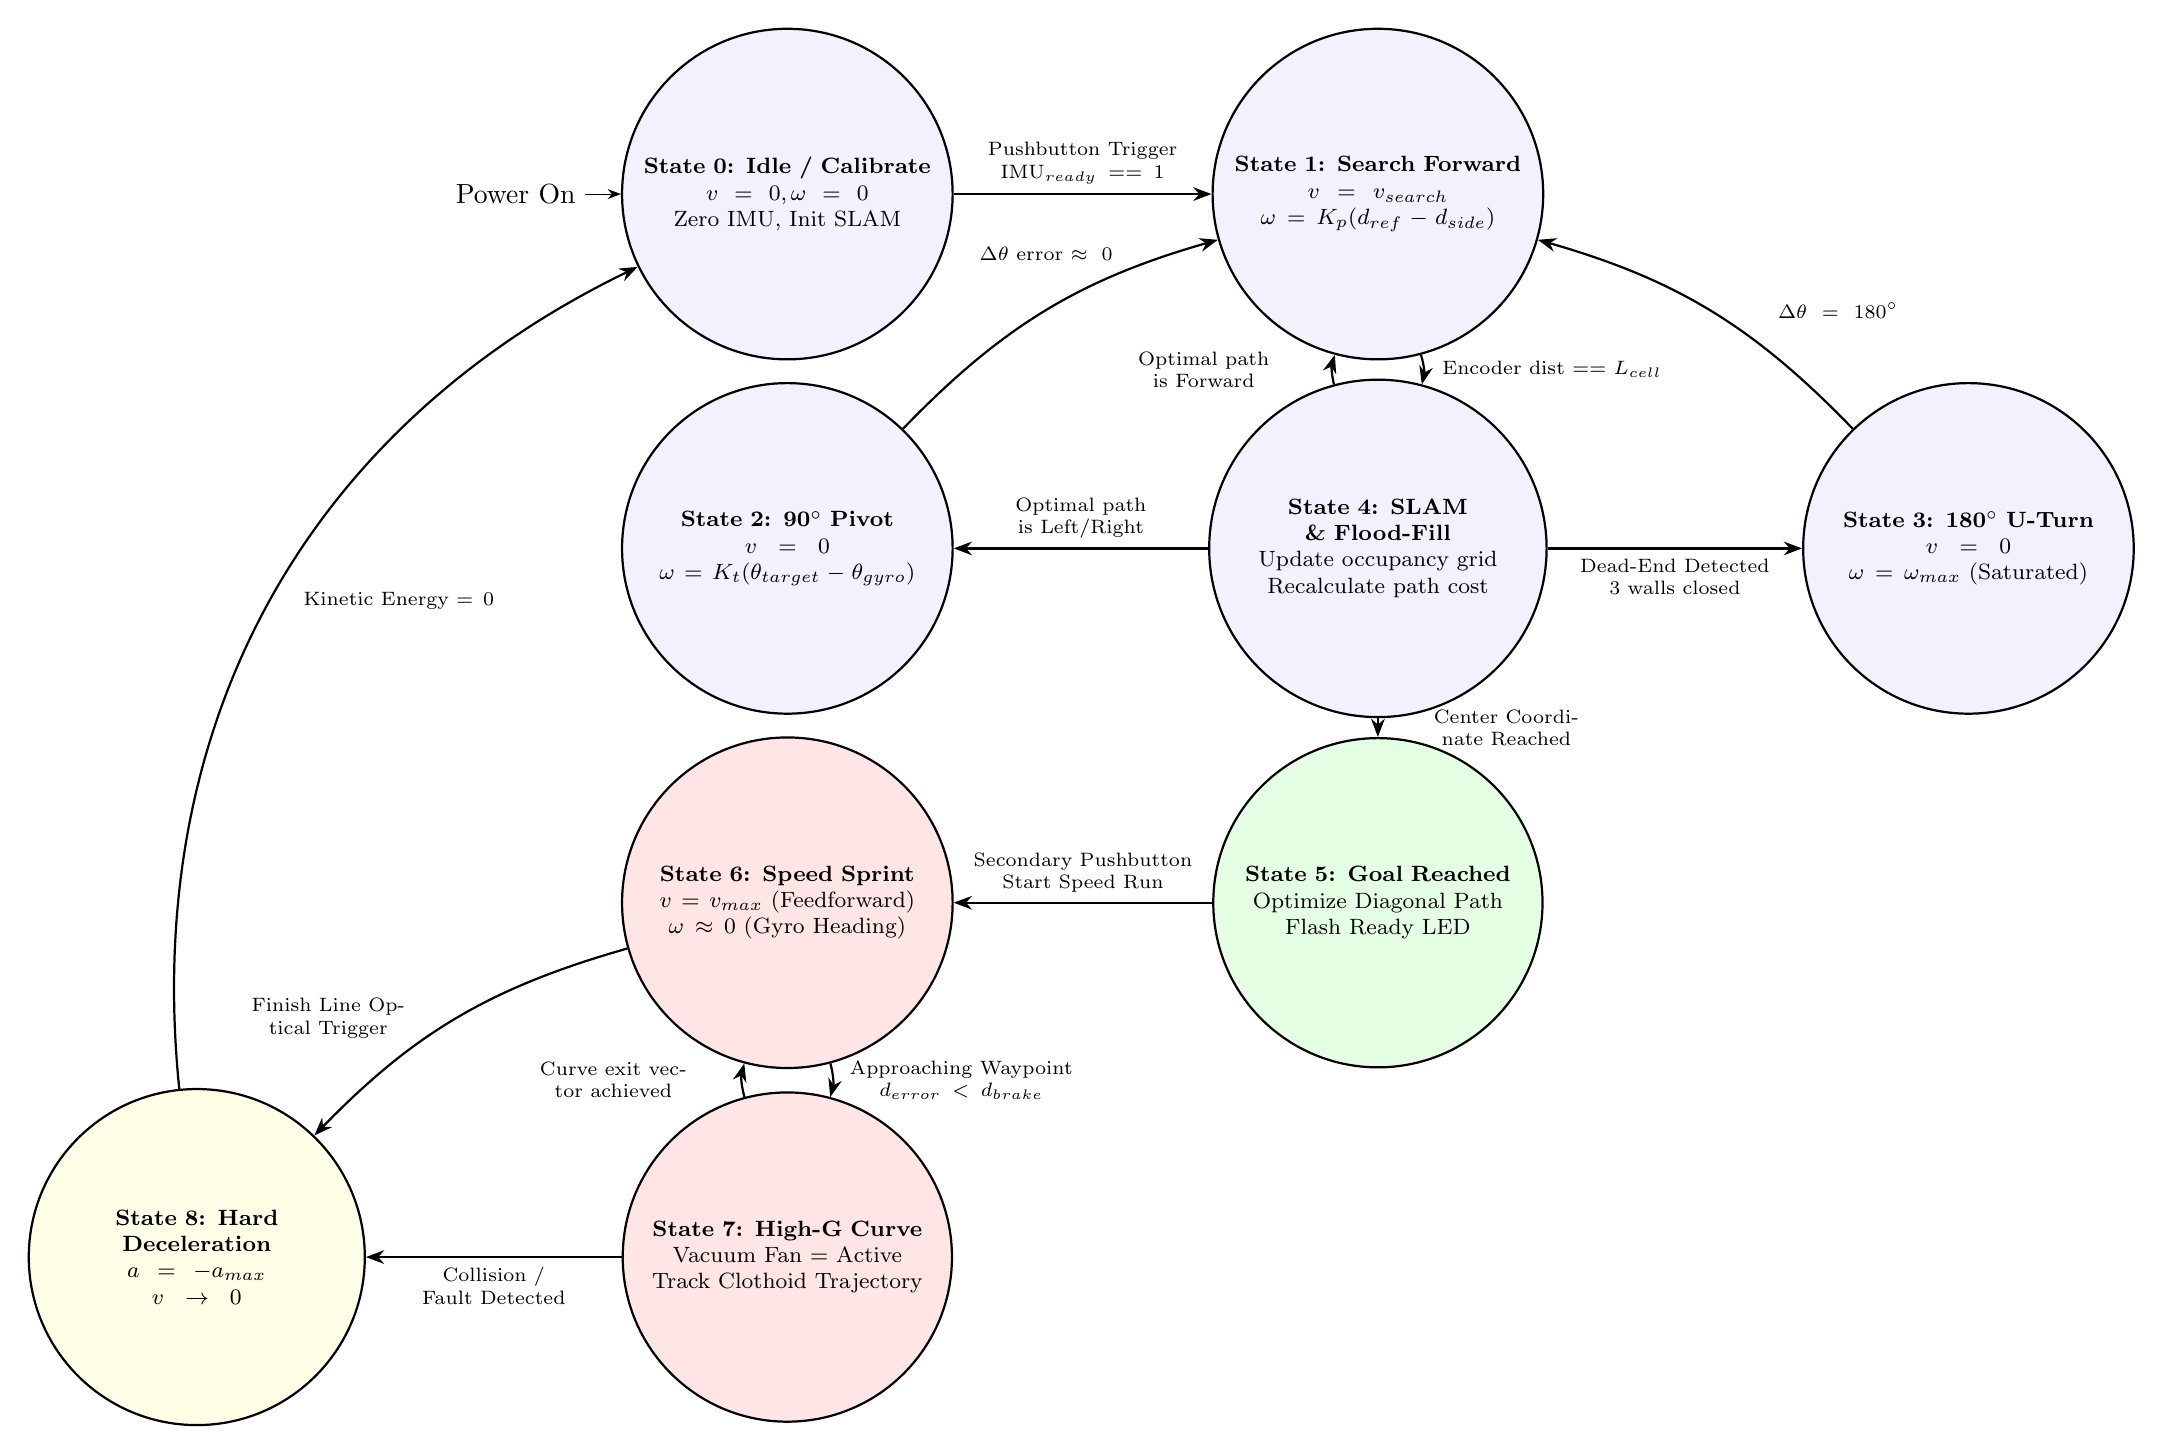
\begin{tikzpicture}[
    >=Stealth,
    node distance=4.5cm and 5.5cm,
    on grid,
    auto,
    every state/.style={thick, fill=blue!5, text width=3.8cm, align=center, font=\footnotesize, minimum height=1.5cm},
    transition/.style={font=\scriptsize, align=center, text width=3cm}
]

% -------------------------
% EXPLORATION STATES
% -------------------------
\node[state, initial, initial text={Power On}] (Idle) {
    \textbf{State 0: Idle / Calibrate}\\ 
    $v=0, \omega=0$\\ 
    Zero IMU, Init SLAM
};

\node[state] (SearchFWD) [right=of Idle, xshift=2cm] {
    \textbf{State 1: Search Forward}\\ 
    $v = v_{search}$\\ 
    $\omega = K_p(d_{ref} - d_{side})$
};

\node[state] (UpdateMap) [below=of SearchFWD] {
    \textbf{State 4: SLAM \& Flood-Fill}\\ 
    Update occupancy grid\\
    Recalculate path cost
};

\node[state] (SearchTurn) [left=of UpdateMap, xshift=-2cm] {
    \textbf{State 2: 90$^\circ$ Pivot}\\ 
    $v = 0$\\ 
    $\omega = K_t(\theta_{target} - \theta_{gyro})$
};

\node[state] (SearchUTurn) [right=of UpdateMap, xshift=2cm] {
    \textbf{State 3: 180$^\circ$ U-Turn}\\ 
    $v = 0$\\ 
    $\omega = \omega_{max}$ (Saturated)
};

\node[state, fill=green!10] (Goal) [below=of UpdateMap] {
    \textbf{State 5: Goal Reached}\\ 
    Optimize Diagonal Path\\
    Flash Ready LED
};

% -------------------------
% SPEED RUN STATES
% -------------------------
\node[state, fill=red!10] (SpeedStraight) [left=of Goal, xshift=-2cm] {
    \textbf{State 6: Speed Sprint}\\ 
    $v = v_{max}$ (Feedforward)\\ 
    $\omega \approx 0$ (Gyro Heading)
};

\node[state, fill=red!10] (SpeedDiag) [below=of SpeedStraight] {
    \textbf{State 7: High-G Curve}\\ 
    Vacuum Fan = Active\\
    Track Clothoid Trajectory
};

\node[state, fill=yellow!10] (Brake) [left=of SpeedDiag, xshift=-2cm] {
    \textbf{State 8: Hard Deceleration}\\ 
    $a = -a_{max}$\\ 
    $v \rightarrow 0$
};

% -------------------------
% TRANSITIONS
% -------------------------
% Idle to Search
\path[->, thick]
(Idle) edge node [transition, above] {Pushbutton Trigger\\ $\text{IMU}_{ready} == 1$} (SearchFWD);

% Search Loops
\path[->, thick]
(SearchFWD) edge [bend left=15] node [transition, right] {Encoder dist == $L_{cell}$} (UpdateMap)
(UpdateMap) edge [bend left=15] node [transition, left] {Optimal path is Forward} (SearchFWD);

\path[->, thick]
(UpdateMap) edge  node [transition, above] {Optimal path is Left/Right} (SearchTurn)
(SearchTurn) edge [bend right=-15] node [transition, above=0.5cm] {$\Delta\theta$ error $\approx 0$} (SearchFWD);

\path[->, thick]
(UpdateMap) edge node [transition, below] {Dead-End Detected\\ 3 walls closed} (SearchUTurn)
(SearchUTurn) edge [bend left=-15] node [transition, right] {$\Delta\theta = 180^\circ$} (SearchFWD);

% Goal and Speed Run
\path[->, thick]
(UpdateMap) edge node [transition, right] {Center Coordinate Reached} (Goal)
(Goal) edge node [transition, above] {Secondary Pushbutton\\ Start Speed Run} (SpeedStraight);

% Speed Run Kinematics
\path[->, thick]
(SpeedStraight) edge [bend left=15] node [transition, right] {Approaching Waypoint\\ $d_{error} < d_{brake}$} (SpeedDiag)
(SpeedDiag) edge [bend left=15] node [transition, left] {Curve exit vector achieved} (SpeedStraight);

% Braking
\path[->, thick]
(SpeedStraight) edge [bend right=15] node [transition, left] {Finish Line Optical Trigger} (Brake)
(SpeedDiag) edge node [transition, below] {Collision / Fault Detected} (Brake)
(Brake) edge [bend right=-35] node [transition, right] {Kinetic Energy $= 0$} (Idle);

\end{tikzpicture}
\end{document}